
%\chapter{Introduction}

\chapter{Introducere}
\label{cap:Introducere}


\section{Context}

În general, tentativele de exploatare a vulnerabilităților unei aplicații vin sub formă de input către aceasta, input generat de către un atacator care intenționează să întrerupă activitatea sau să preia controlul aplicației. Un sistem de prevenire a intruziunilor (IPS) este poziționat între aplicație și clienții acesteia, și previne exploatarea unor astfel de vulnerabilități. 

Prin folosirea unui reverse proxy pentru accesarea resurselor unui server de către clienți, se poate să se aducă numeroase beneficii procesului de administrare a serverului \cite{top_8}. Spre deosebire de un forward proxy care e un intermediar pentru o serie de clienți prestabiliți, pentru a accesa orice server, un reverse proxy e un intermediar pentru o serie de servere prestabilite pentru a fi accesate de orice client. Unul dintre avantajele folosirii unui reverse proxy este centralizarea întregului trafic al serverului/serverelor într-un singur punct de acces, aceasta fiind și principala caracteristică exploatată de acest proiect pentru filtrarea IP-urilor nedorite (în cazul nostru cele utilizate de rețeaua Tor) și verificarea conţinutului URI-urilor pentru posibile atacuri (SQL injection).

\begin{figure}[h]
	\centering
	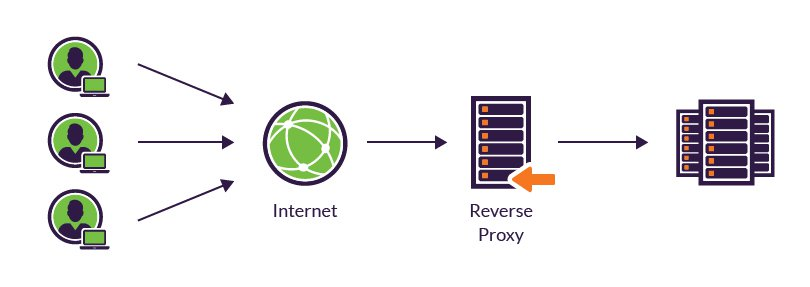
\includegraphics[width=0.5\textwidth]{reverse-proxy-02-1.jpg}
	\caption{ Diagramă reverse proxy }
	\label{fig:reverse-proxy}
\end{figure}

Figura ~\ref{fig:reverse-proxy}  ilustrează modul de funcționare al unui reverse proxy în relație cu serverele aferente și posibili clienți.  \\

 

Conform topului alcătuit de fundația OWASP cu cele mai mari 10 riscuri ale aplicațiilor în 2017 \cite{owasp}, SQL injection e considerat a fi cea mai mare vulnerabilitate a aplicațiilor web. Acest lucru se datorează faptului că mare parte din aceste aplicații se bazează pe procesarea conținutului furnizat de către utilizatori. Atacurile de tipul SQL injection constau în faptul că datele furnizate de către utilizator sunt introduse în interogări SQL, unde acestea sunt tratate că și cod executabil \cite{classification_and_countermeasures}. Aplicațiile web vulnerabile la SQLi injection pot permite unor utilizatori neautorizați să facă interogări într-o bază de date, asupra unor date la care nu ar avea acces în mod normal. Folosind acest tip de comportament neautorizat, un astfel de utilizator poate să obțină accesul la informații sensibile ale clienților, dar și a administratorilor aplicației, precum credențiale sau date personale. Această vulnerabilitate poate să ducă la furt de identitate sau fraudă.  
 
În cazul rețelei Tor, aceasta le permite utilizatorilor să navigheze pe internet anonim. Anonimitatea online este importantă însă în multe cazuri aplicațiile web trebuie să știe cine se conectează la aceasta pentru a le putea determina intențiile. Numele de Tor vine de la "the onion router" care sugerează modul de operare al rețelei. Fiecare participant la rețea devine un nod de transfer, iar traficul rețelei traversează o serie de astfel noduri până să ajungă la nodul de ieșire ce creează conexiunea cu destinația dorită. Pachetele sunt criptate în mai multe "straturi", fiecare nod decriptand un singur strat de unde poate afla doar destinația nodului următor. Când pachetul ajunge la ultimul nod, acesta trimite conținutul la destinație fără să dezvăluie identitatea sursei. Această anonimitate ușurează desfășurarea atacurilor online. Conform datelor din rețeaua organizației CloudFlare 94\% din traficul provenit din rețeaua Tor este alcătuit din request-uri automate de origine malițioasă \cite{tor_trouble}. 

%\section{Motivation}
 \section{Motivație}
În piața actuală există multe sistem de prevenire a intruziunilor ce oferă atât caracteristicile unui reverse proxy, cât și cele de securitate. Aceste caracteristici sunt oferite fie ca și produse individuale, fie ca și produse ce le încorporează pe ambele. Cu toate acestea, produsele de acest gen sunt în general scumpe, au o logică mascată de detectare a posibilelor probleme de securitate și sunt greu de înțeles și de configurat de către utilizator după propriile nevoi. 

Prin oferirea utilizatorilor posibilitatea de a configura modul de funcționare a unui astfel de sistem, poate rezulta în sisteme mult mai eficiente și rapide, dedicate pentru preferințele și nevoile aplicației fiecărui utilizator în parte. Spre exemplu, un utilizator poate să decidă că nu are nevoie de funcționalitățile de detecție împotrivă atacurilor de tip SQL injection pentru o anumită aplicație, întrucât aceasta nu prezintă vulnerabilități din acest punct de vedere, nefolosind baze de date. În cazul acesta prin eliminarea unui astfel de modul, se elimină și verificările aferente asupra request-urilor clienților, îmbunătățind astfel performanțele sistemului. 

\textit{\thesistitle}  oferă un sistem configurabil după preferințele utilizatorilor. Utilizatorul poate configura detecția bazată pe analiză request-ului primit de la client, acesta poate să aleagă care module să fie folosite pentru detecție, permițând și eventuala adăugare de noi module (cât timp acestea respectă anumite condiții de structură), meniurile din interfața utilizator fiind generate în mod dinamic în funcție de modelele prezente. Utilizatorul poate, de asemenea să configureze și lista IP-urilor blocate, permițându-i-se să șteargă din cele existente, respectiv să adauge unele noi, după bunul plac. 


%\section{Report's Structure}
 \section{Structura lucrării}
În această secțiune se prezintă structura lucrării pe capitole și o scurtă descriere a conținutului acestora: 

Primul \textbf{capitol} ~\ref{cap:Introducere},  prezintă o scurtă introducere despre proiect, contextul acestuia și motivația pentru implementarea sistemului propus. 

\textbf{Capitolul}~\ref{cap:obiective-specificatii}  prezintă obiectivele lucrării, specificațiile sistemului, motivând deciziile luate în implementarea sistemului, cerințele funcționale și non-funcționale necesare implementării sistemului. 

\textbf{Capitolul}~\ref{cap:studiu-bibliografic}  descrie alte abordări similare ale problemelor tratate de proiectul propus, prin evidențierea asemănărilor și diferențelor dintre acestea și se explică tehnologiile și metodele folosite de proiect. 
 
In \textbf{capitolul}~\ref{cap:fund-teoretice}  sunt evidențiate și explicate pe scurt aspectele teoretice pe care se bazează proiectul.

\textbf{Capitolul}~\ref{cap:analiza-si-proiectare}  descrie design-ul proiectului și cuprinde: cerințele sistemului, specificațiile cazurilor de utilizare, arhitectura sistemului, comportamentul sistemului, datele utilizate de sistem, dependințele sistemului, algoritmi esențiali și metodele folosite. Descrierea acestora se realizează prin asocierea cu diagramele aferente.


\textbf{Capitolul}~\ref{cap:implementare}  prezintă în amănunt detaliile de implementarea a proiectului. În acest capitol sunt abordate: organizarea codului sursă, descrierea principalelor clase și funcționalități ale proiectului și posibilitățile de desfășurare a execuției programului. 

\textbf{Capitolul} ~\ref{cap:rezultate}  reprezintă metodele de validare a soluțiilor/sistemului descris în capitolele anterioare, scenariile de testare a corectitudinii funcționale, a utilizabilității și performanței. 

\textbf{Capitolul}~\ref{cap:user-manual} descrie pașii de instalare și rulare a aplicației.

\textbf{Capitolul}~\ref{cap:concluzii} cuprinde ce s-a realizat, relativ la ce s-a propus, în ce constă experiența acumulată, care au fost punctele dificile atinse și o descriere a posibilelor dezvoltări și îmbunătățiri ulterioare.